\chapter{Funzioni}

\begin{definition}[Funzione]
    Presi due insiemi $x$ e $y$ una funzione $f:x\rightarrow y$ è una legge che ad ogni elemento di $x$ associa un elemento di $y$.
\end{definition}
\begin{figure}[ht]
    \centering
    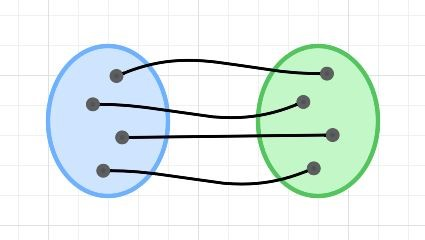
\includegraphics[width = 6cm]{images/funzioni.JPG}
    \caption{Esempio insiemistico di una funzione}
    \label{fig:funzioni}
\end{figure}
$f:x\rightarrow y, x\longmapsto f(x)$
\begin{definition}[Funzione immagine]
    L'insieme immagine di $f$, $Im(f)=\{f(x):x\in X\}$ sono tutti gli elementi di $f$.
\end{definition}
\begin{definition}[Funzione reale]
    Se $x, y \subset\mathbb{R}, fx\rightarrow y$ si dice funzione reale a variabile reale.
\end{definition}

L'analisi matematica si occupa proprio dello studio delle funzioni reali a variabile reale.

\section*{Il grafico della funzione}
Notiamo come la rappresentazione insiemistica (\ref{fig:funzioni}) è possibile solo con pochi elementi. A tal proposito possiamo rappresentare una funzione su una regione molto più ampia come il nostro piano con due assi chiamati per l'appunto assi cartesiani.
\begin{example}[Funzione modulo]
    $|.|:\mathbb{R}\rightarrow\mathbb{R}, x\longmapsto |x|$\\
    \begin{tikzpicture}
    \begin{axis}[xmin=-5,xmax=5,ymin=-3,ymax=3,
    axis x line=middle,
    axis y line=middle]
    \addplot [very thick, 
        domain=-10:10,
        samples=500, 
        color=magenta,
    ]
    {abs(x)};
    \addlegendentry{\(|x|\)}
    \end{axis}
    \end{tikzpicture}
    
    La funzione è simmetrica e è limitata verso il basso.
\end{example}

\section{Funzioni composte}
Fin ora abbiamo visto che una funzione si definisce come una relazione tra dominio e codominio. Ma perchè non mettere in relazione una funzione con un'altra e un'altra ancora?

Supponiamo di avere due funzioni $f:x\rightarrow y$ e $g:w\rightarrow z$ t.c. $f(x)\subset w$.

\begin{figure}[ht]
    \centering
    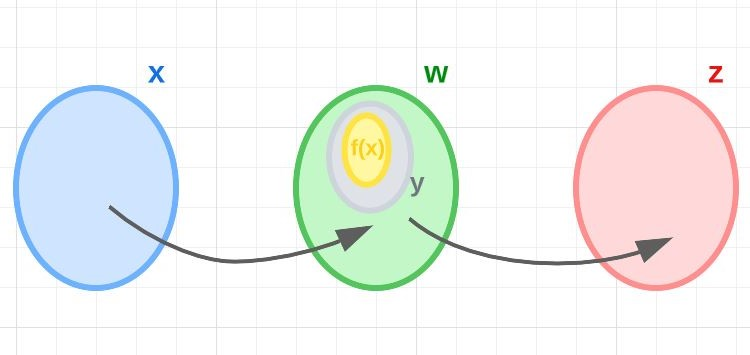
\includegraphics[width = 9cm]{images/composizione_funz.JPG}
    \caption{Composizione di funzioni}
    \label{fig:comp_funz}
\end{figure}
\begin{equation}
    g\circ f:x\rightarrow z,  x\longmapsto g(f(x))
\end{equation}

\begin{example}
    Prendiamo due funzioni $sin$ e $|.|:\mathbb{R}\rightarrow\mathbb{R}$, $x\longmapsto sin(|x|)$
    
    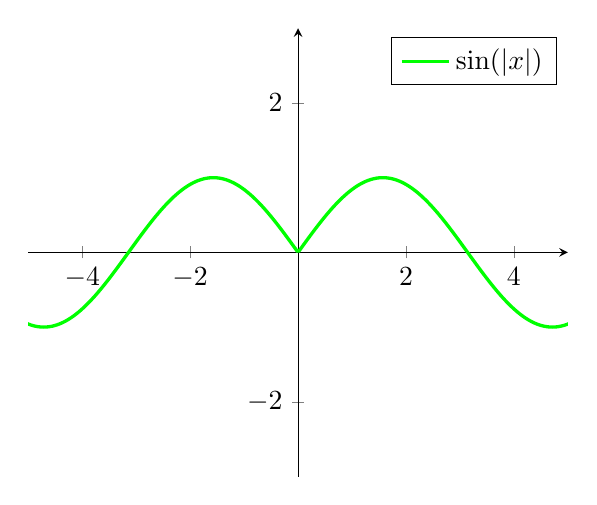
\begin{tikzpicture}
    \begin{axis}[xmin=-5,xmax=5,ymin=-3,ymax=3,
    axis x line=middle,
    axis y line=middle]
    \addplot [very thick, domain=-10:10, samples=500, color=green,]{sin(deg(abs(x)))};\addlegendentry{\(\sin(|x|)\)}
    \end{axis}
    \end{tikzpicture}
    
\end{example}

Ovviamente è possibile anche il procedimento inverso, ovvero partire da una funzione composta e deriverne la singole funzioni che la compongono.

\section{Operazioni tra funzioni}
Date $f$ e $g$ con lo stesso dominio, posso definire $f+g$ e $f*g$ come:\\$(f+g)(x)=f(x)+g(x)\hspace{0,5cm}(fg)(x)=f(x)g(x)$

\section{Dominio naturale}
\begin{definition}[Dominio naturale]
    Il dominio naturare è il più grande $x\subseteq\mathbb{R}$ t.c. $f$ è ben definita su $x$.
\end{definition}

Se il dominio naturale non è presente, sarà rappresentato dall'insime  naturale più ampio su cui è possibile definire una funzione.

\begin{example}
    $f(x)=\ln(x^2-4)$\\$x^2-4>0\hspace{0,5cm}x^2>4\hspace{0,5cm}x<-2\lor x>2$
    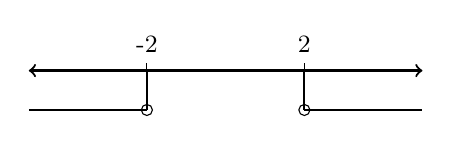
\begin{tikzpicture}
    \draw[<->,thick] (0,0) -- (5,0);
    \draw (1.5,0) -- (1.5,0.1) node [above] {\small{-2}};
    \draw (3.5,0) -- (3.5,0.1) node [above] {\small{2}};
    \draw[black] (1.5,-0.5) circle (2pt);
    \draw[black] (3.5,-0.5) circle (2pt);
    \draw[-,thick] (0,-0.5) -- (1.5,-0.5);
    \draw[-,thick] (3.5,-0.5) -- (5,-0.5);
    \draw[-,thick] (1.5,-0) -- (1.5,-0.5);
    \draw[-,thick] (3.5,-0) -- (3.5,-0.5);
\end{tikzpicture}
\end{example}

\section{Tipi di funzioni}
\subsection*{Iniettiva}
\begin{definition}[Iniettiva]
    $f:x\rightarrow y$ si dice iniettiva se $x_1\neq x_2\Rightarrow f(x_1)\neq f(x_2)$.
\end{definition}

Per semplificare una funzione si dice iniettiva quando ad ogni elemento $x$ corrisponde uno e un solo punto di $f(x)$.

La funzione espoenenziale è un esempio di funzione iniettiva mentre la funzione $\cos$ non lo è.

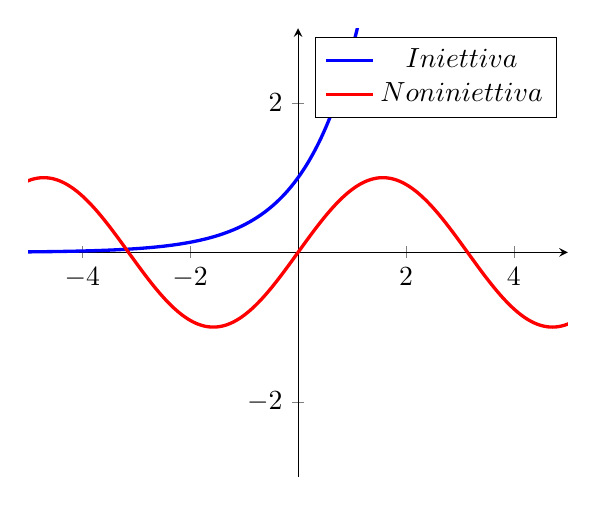
\begin{tikzpicture}
    \begin{axis}[xmin=-5,xmax=5,ymin=-3,ymax=3,
    axis x line=middle,
    axis y line=middle]
    \addplot [very thick, domain=-5:5, samples=500, color=blue,]{e^x};\addlegendentry{\(Iniettiva\)}
    \addplot [very thick, domain=-10:10, samples=500, color=red,]{sin(deg(x))};\addlegendentry{\(Non iniettiva\)}
    \end{axis}
\end{tikzpicture}

\subsection*{Surriettiva}
\begin{definition}[Surriettiva]
    $fx\rightarrow y$ si dice surriettiva se $f(x)=y$
\end{definition}

Ovvero se ogni punto di $y$ viene prima o poi raggiunto da una freccia ovvero ad ogni elemento di $y$ corrisponde almeno un elemento di $x$.

Quindi la funzione $\ln(0,+\infty)$ è surriettiva mentre la funzione $e^x$ non lo è perchè i punti $\leq 0$ non vengono mai presi.

\subsection*{Inversa}
\begin{definition}[Inversa]
    Se $fx\rightarrow y$ è iniettiva $f^{-1}:f(x)\rightarrow x, y\longmapsto x$ t.c. $f(x)=y$ la funzione si chiama inversa di $f$.
\end{definition}

Ovvero se la funzione è iniettiva, per ogni elemento di $x$ corrisponde un elemento di $y$ e viceversa.

\begin{example} La funzione $f[0+\infty)\rightarrow\mathbb{R},  x\longmapsto x^2$ è una funzione invertibile.
    La sua inversa è $f^{-1}(x)=\sqrt{x}$
    
    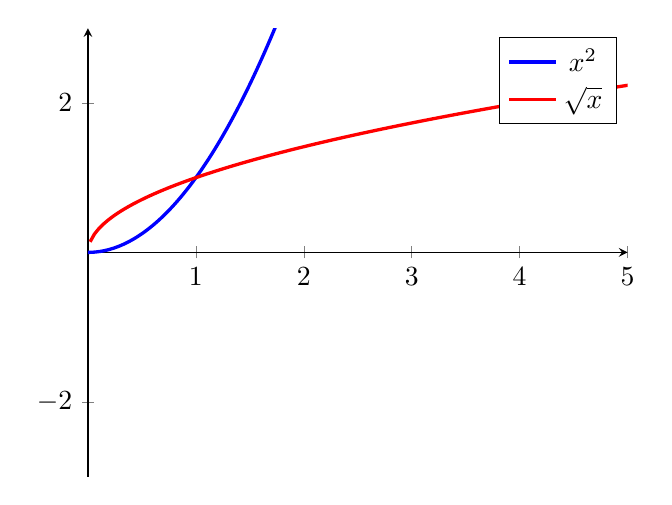
\begin{tikzpicture}
        \begin{axis}[xmin=0,xmax=5,ymin=-3,ymax=3,
        axis x line=middle,
        axis y line=middle]
        \addplot [very thick, domain=-5:5, samples=500, color=blue,]{x^2};\addlegendentry{\(x^2\)}
        \addplot [very thick, domain=-10:10, samples=500, color=red,]{sqrt(x)};\addlegendentry{\(\sqrt{x}\)}
        \end{axis}
    \end{tikzpicture}
    
\end{example}

\subsection*{Pari e dispari}
\begin{definition}[Pari]
    $fx\rightarrow y, x,y\in\mathbb{R}$ si dice pari se $f(x)=f(-x),\forall x\in\mathbb{R}$
\end{definition}
$f(x)=x^2$ è una funzione pari, simmetrica rispetto all'asse y.
\begin{definition}[Dispari]
    $fx\rightarrow y, x,y\in\mathbb{R}$ si dice dispari se $f(x)=-f(x),\forall x\in\mathbb{R}$
\end{definition}
$f(x)=x^3$ è una funzione dispari, simmetrica rispetto al punto di coordinate $(0,0)$.

\subsection*{Monotona}
\begin{definition}[Crescente]
    $fx\rightarrow y, x,y\in\mathbb{R}$ si dice monotona crescnte se $x_1<x_2\Rightarrow f(x_1)<f(x_2)$
\end{definition}

\begin{tikzpicture}
    \begin{axis}[xmin=-5,xmax=5,ymin=-3,ymax=3,
    axis x line=middle,
    axis y line=middle]
    \addplot [very thick, domain=-5:5, samples=500, color=cyan,]{e^x};\addlegendentry{\(e^x\)}
    \end{axis}
\end{tikzpicture}

\begin{definition}[Descrescente]
    $fx\rightarrow y, x,y\in\mathbb{R}$ si dice decrescnte se $x_1<x_2\Rightarrow f(x_1)>f(x_2)$    
\end{definition}

\begin{tikzpicture}
    \begin{axis}[xmin=-5,xmax=5,ymin=-3,ymax=3,
    axis x line=middle,
    axis y line=middle]
    \addplot [very thick, domain=-5:5, samples=500, color=magenta,]{(0.5)^x};\addlegendentry{\((\frac{1}{2})^x\)}
    \end{axis}
\end{tikzpicture}

\begin{description}
		\item[N.B.]  Le funzioni crescenti e decrescenti sono sempre iniettive.
\end{description}

\subsection*{Periodica}
\begin{definition}[Periodica]
    $fx\rightarrow y$ con $x,y\in\mathbb{R}$ si dice periodica se $\exists T>0$ t.c. $f(x+T)=f(x), \forall x\in\mathbb{R}$.
\end{definition}
Il più piccolo intervallo di $T$ viene chiamato periodo della funzione.

Le funzioni $\sin$ e $\cos$ sono funzioni periodiche.

\subsection*{Trigonometriche}
In breve, presa una circonferenza goniometrica e un angolo $\alpha$ possiamo determinare il $\sin$ e $\cos$ grazie agli angoli in radianti:

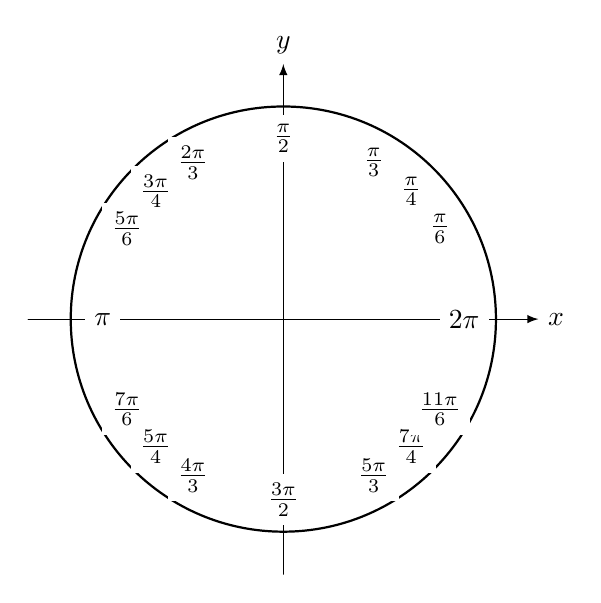
\begin{tikzpicture}[scale=2.7,cap=round,>=latex]
        % draw the coordinates
        \draw[->] (-1.2cm,0cm) -- (1.2cm,0cm) node[right,fill=white] {$x$};
        \draw[->] (0cm,-1.2cm) -- (0cm,1.2cm) node[above,fill=white] {$y$};

        % draw the unit circle
        \draw[thick] (0cm,0cm) circle(1cm);
        % draw the radiant
        \foreach \x/\xtext in {
            30/\frac{\pi}{6},
            45/\frac{\pi}{4},
            60/\frac{\pi}{3},
            90/\frac{\pi}{2},
            120/\frac{2\pi}{3},
            135/\frac{3\pi}{4},
            150/\frac{5\pi}{6},
            180/\pi,
            210/\frac{7\pi}{6},
            225/\frac{5\pi}{4},
            240/\frac{4\pi}{3},
            270/\frac{3\pi}{2},
            300/\frac{5\pi}{3},
            315/\frac{7\pi}{4},
            330/\frac{11\pi}{6},
            360/2\pi}
                \draw (\x:0.85cm) node[fill=white] {$\xtext$};
            % draw the sin e cos
\end{tikzpicture}
$\cos^2x+\sin^2x=1$

Ecco quindi i grafici delle funzioni prese in oggetto:

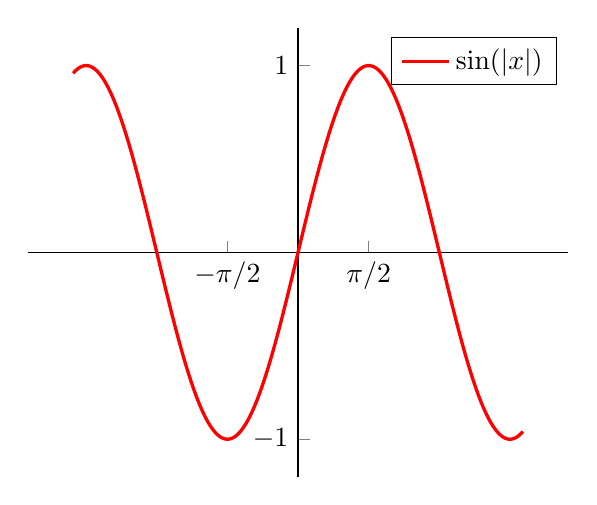
\begin{tikzpicture}
    \begin{axis}[domain=-1:1, samples=500, axis lines*=middle, ytick={-1,1}, xtick={-1.57,1.57}, xticklabels={$-\pi$/2,$\pi$/2}];
    \addplot [very thick, domain=-5:5, samples=500, color=red,]{sin(deg(x))};\addlegendentry{\(\sin(|x|)\)}
    \end{axis}
\end{tikzpicture}

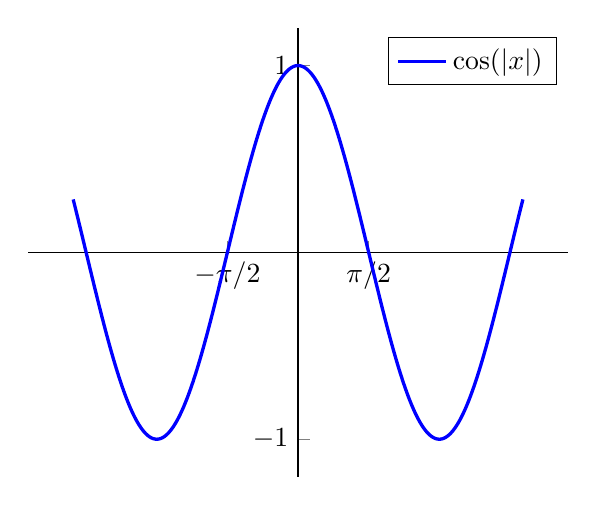
\begin{tikzpicture}
    \begin{axis}[domain=-1:1, samples=500, axis lines*=middle, ytick={-1,1}, xtick={-1.57,1.57}, xticklabels={$-\pi$/2,$\pi$/2}];
    \addplot [very thick, domain=-5:5, samples=500, color=blue,]{cos(deg(x))};\addlegendentry{\(\cos(|x|)\)}
    \end{axis}
\end{tikzpicture}

\subsubsection{Trigonometriche inverse}
Considerando intervalli più piccoli come nel caso del $\sin|[-\frac{\pi}{2},\frac{\pi}{2}]\rightarrow [-1+1]$ noto che posso ugualmente rappresentarlo. Essendo un intervallo finito posso affermare con certezza che la funzione è iniettiva e quindi invertibile.
La funzione inversa del $\sin$ è:

\begin{tikzpicture}
  \begin{axis}[domain=-1:1, samples=500, axis lines*=middle, xtick={-1,1}, ytick={-1.57,1.57}, yticklabels={$-\pi$/2,$\pi$/2}];
  \addlegendentry{\(\arcsin(x)\)}
    \addplot[very thick, color = red]  {asin(x)/180*pi};
      \end{axis}
\end{tikzpicture}

Lo stesso procedimento è applicabile con la funzione $\cos$. Ne risulterà la funzione $\cos|[0,\pi]\rightarrow [-1+1]$
La funzione inversa del $\cos$ è:

\begin{tikzpicture}
  \begin{axis}[domain=-1:1, samples=500, axis lines*=middle, xtick={-1,1}, ytick={-1.57,1.57}, yticklabels={$-\pi$/2,$\pi$/2}];
  \addlegendentry{\(\arccos(x)\)}
    \addplot[very thick, color = blue]  {acos(x)/180*pi};
      \end{axis}
\end{tikzpicture}

Senza discriminare le precedenti funzioni possiamo dire però che la funzione trigonometrica inversa più importate è sicuramnte l'$\arctan$.

Ma diamo prima un ripasso della funzione $\tan$.
\begin{equation}
    tanx=\frac{sinx}{cosx}
\end{equation}

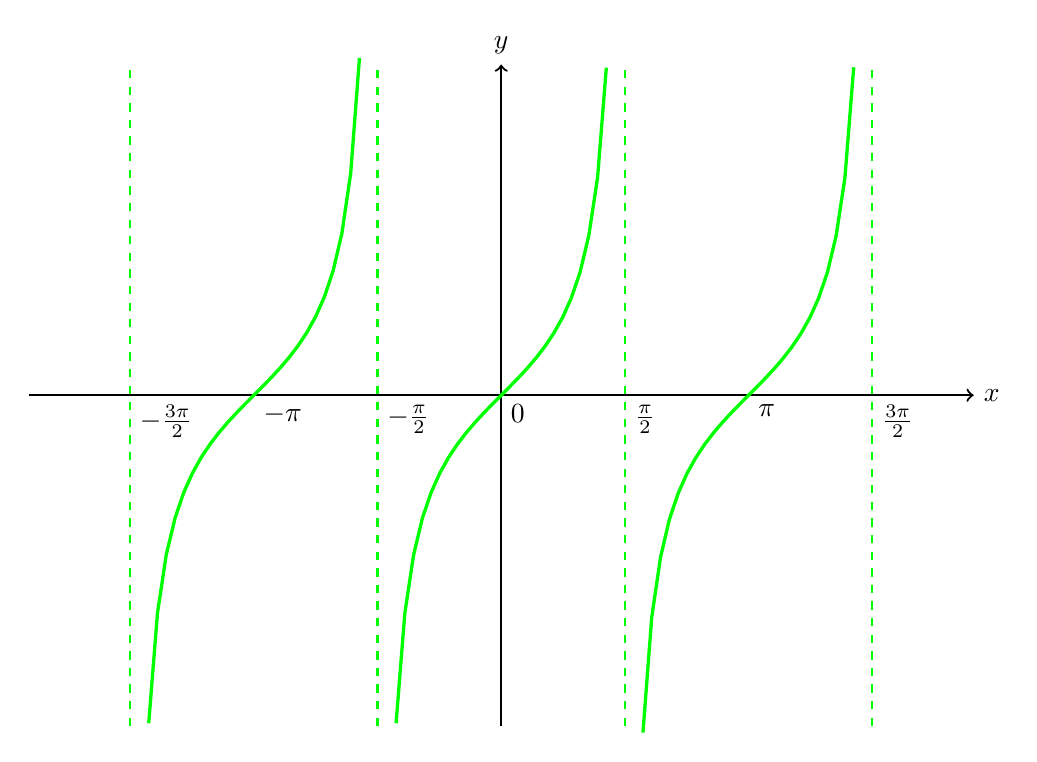
\begin{tikzpicture}[domain=-4:7] [scale=0.8]
% x and y axes
\draw[thick, ->] (-6,0)     -- (6,0)   node[right] {$x$};
\draw[thick, ->] (0,-4.2)   -- (0,4.2) node[above] {$y$};
% vertical asymptotes
\draw[dashed, thick,green] (pi/2,-4.2)    --  (pi/2,4.2);
\draw[dashed, thick,green] (3*pi/2,-4.2)  --  (3*pi/2,4.2);
\draw[dashed, thick,green] (-pi/2,-4.2)   --  (-pi/2, 4.2);
\draw[dashed, thick,green] (-3*pi/2,-4.2) --  (-3*pi/2, 4.2);
% tangent between vertical asymptotes
\draw[very thick,color=green, -] plot [domain=-0.425*pi:0.425*pi] (\x,{tan(\x r)});
\draw[very thick,color=green, -] plot [domain= 0.573*pi:1.425*pi] (\x,{tan(\x r)});
\draw[very thick,color=green, -] plot [domain= -1.425*pi:-0.573*pi] (\x,{tan(\x r)});
% x tick labels
\node[below right] at (-3*pi/2, 0)  {$-\frac{3\pi}{2}$};
\node[below right] at (-pi, 0)      {$-\pi$};
\node[below right] at (-pi/2, 0)    {$-\frac{\pi}{2}$};
\node[below right] at (0, 0)        {$0$};
\node[below right] at (pi/2, 0)     {$\frac{\pi}{2}$};
\node[below right] at (pi, 0)       {$\pi$};
\node[below right] at (3*pi/2, 0)   {$\frac{3\pi}{2}$};
\end{tikzpicture}

Ovviamente una funzione di questo tipo non può essere iniettiva, quindi la restringo in intervallo come mostrato prima.
Una volta invertita la funzione si ottiene: $tan|(-\frac{\pi}{2},\frac{\pi}{2})$.

\begin{tikzpicture}
  \begin{axis}[domain=-1:1, samples=500, axis lines*=middle, xtick={-1,1}, ytick={-1.57,1.57}, yticklabels={$-\pi$/2,$\pi$/2}, xticklabels={$-\infty$,$\infty$}];
  \addlegendentry{\(\arctan(x)\)}
    \addplot[very thick, color = green]  {atan(x)/180*pi};
      \end{axis}
\end{tikzpicture}

Come tale il procedimento di inversione è sempre applicabile anche ad esempio con la funzione cotangente:
\begin{equation}
    cotx=\frac{cosx}{sinx}
\end{equation}

\subsection*{Iperboliche}
\begin{definition}[Funzioni iperboliche]
    Il $\sin$ iperbolico di $\sin hx=\frac{e^x-e^{-x}}{2}$
    
    Il $\sin$ iperbolico di $\cos hx=\frac{e^x+e^{-x}}{2}$
\end{definition}

Che formule complesse!!! Vediamo di semplificarle un pò:
\begin{osservation}
    $-\sin h^2x+\cos h^2x$\\
    $-(\frac{e^x-e^{-x}}{2})^2+(\frac{e^x-e^{-x}}{2})^2$\hspace{1cm}$-\frac{(e^x)^2-2e^xe^{-x}+(e^{-x})^2}{4}+\frac{(e^x)^2+2e^xe^{-x}+(e^{-x})^2}{4}$\\
    $-\frac{e^{2x}-2e^0+e^{-2x}}{4}+\frac{e^{2x}-2e^0+e^{-2x}}{4}$\hspace{1cm}$\frac{-e^{2x}+2-e^{2x}+2+e^{2x}}{4}$\\
    Semplificando otteniamo $\frac{4}{4}=1$
\end{osservation}
